\documentclass{article}

\usepackage[margin=1in]{geometry}
\usepackage{amsmath}
\usepackage{amssymb}
\usepackage{amsthm}
\usepackage{graphicx}
\theoremstyle{definition}
\newtheorem{definition}{Definition}[section]
 
\title{Braid Cryptosystem Notes}
\date{\today}



\begin{document}
	\maketitle
	
	\section{Braid Cryptographic System}
	
	\subsection{Braids}
	%TODO: who created braids and operations on braids
	In this section we will explain the mathematics behind a braid group. A braid group has braids as the set and concatenation as the group operation written as $<B_n,||>$ where $n$ is the number of strands and 

\begin{definition} 
$B_n=\{\sigma_1,...,\sigma_{n-1}:\sigma_i\sigma_j\sigma_i=\sigma_j\sigma_i\sigma_j\ \textrm{if}\ |i-j|=1\ \textrm{and}\ \sigma_i\sigma_j=\sigma_j\sigma_i\ \textrm{if}\ |i-j|>1\}$
\end{definition}
 
A braid group is infinite and nonabelian meaning that the elements do not commute such that:
$a,b \in B_n: \ ab\neq ba$. Note that for $n$ strands there are $n-1$ generators represented by $\sigma$. A braid is the concatenation of generators. A positive generator, $\sigma_i^+$, corresponds to crossing left over right and a negative generator corresponds to crossing right over left, $\sigma_i^-$. 

\begin{figure}[hbp!]
\centering
  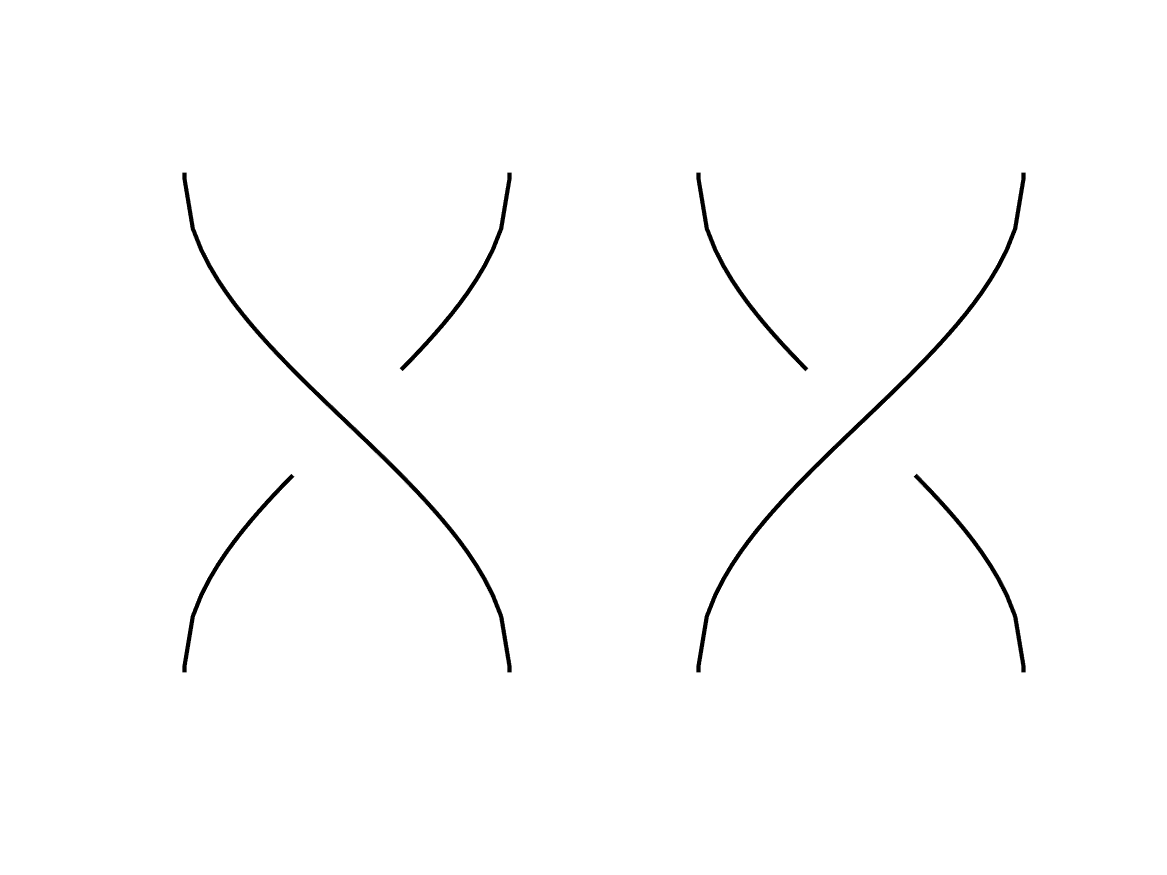
\includegraphics[width=0.2\linewidth]{./Pictures/gen_pos_neg.png}
  \caption{$\sigma_i^+$,$\sigma_i^-$}\label{fig:graph}
\end{figure}


For example the braid $b \in B_3: \ b=\sigma_2^+ \sigma_1^+ \sigma_2^- \sigma_1^-$ is the following:
	
	\begin{figure}[hbp!]
\centering
  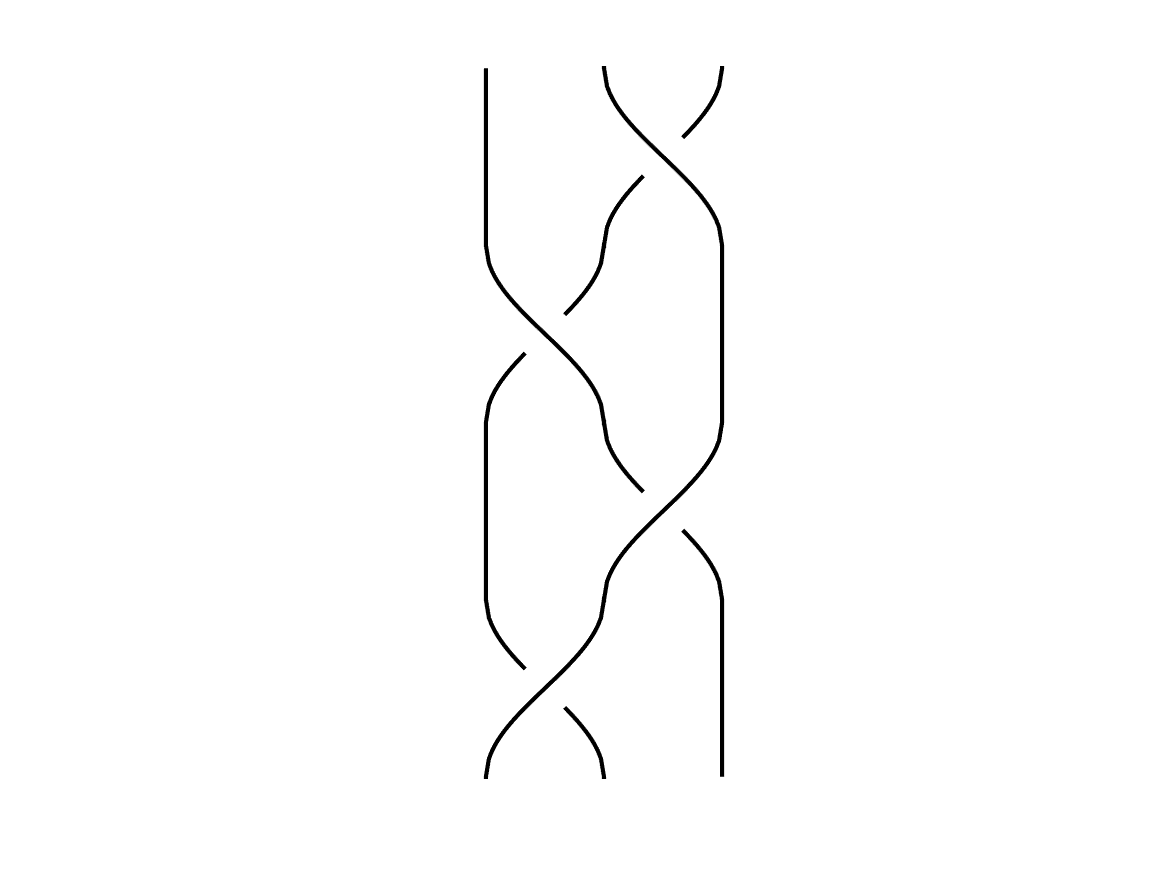
\includegraphics[width=0.2\linewidth]{./Pictures/example_braid.png}
\end{figure}
	
	
	
	
	\subsubsection{Left and Right Canonical Forms}
	
	For any $w \in B_n$ $\exists$ a unique representation called the left canonical form.
	
	\begin{align*}
		&w = \Delta^u A_1 A_2 ... A_l, u \in Z', A \in \Sigma_n \text{ without the following elements } \{ e, \Delta \} \\
		&\text{where } A_i A_{i+1} \text{is left weighted for } 1 \leq i \leq l - 1 \\
		&\text{where } \Sigma_n \text{ is the set of all permutation braids.}
	\end{align*}
	
	\subsection{Hard problem associated with braids.}
	As we have seen in RSA and El-Gamal there are associated hard problems with these crypto systems. For RSA there is the factoring problem where for:
	
	\begin{itemize}
		\item p,q \text{are $2$ distinct k-bit primes.}
		\item n=pq 
		\item \text{Multiplying is computationally easy while the inverse function, factoring, is computationally hard.} 
	\end{itemize}

Similarly El-Gamal has the discrete logarithm which is the associated computationally hard problem. 
For braid group cryptography there are several computationally hard problems. One in particular that is widely used is the conjugacy search problem. Conjugacy is defined as:
\begin{definition} 
$G-\text{group. } a,x,y \in G. \text{ If }y=axa^{-1},\text{ then }y \text{ is } conjugate \text{ to }x \text{ via }a.$
\end{definition}

\noindent \textbf{Conjugacy Search Problem:} \\ $\textbf{Given }x,y \in B_n \text{ such that }y=axa^{-1} \text{ for some }a \in B_n. \\ \textbf{Find }b \in B_n \text{ such that }y=b^{-1}xb.$
\\ \\
There are several types of conjugacy search problems and one we will focus on is the Diffie-Hellman type generalized conjugacy search problem. First we need to define $2$ commuting subgroups of $B_n$. 


\begin{definition}
$LB_n,UB_n < B_n. \\ LB_n=\{ \sigma_1,...,\sigma_{[n/2]-1}  \}, UB_n=\{ \sigma_{[n/2]+1},...,\sigma_{n-1}  \} $
\end{definition}

We know use the fact by definition of a braid group that generators commute if and only if the generators do not share a common strand. Since the $\sigma_{n/2}$ generator is missing, elements in each subgroup will commute with each other such that: $a \in LB_n, b \in UB_n, ab=ba$. We can know look at the Diffie-Hellman generalized conjugacy search problem.
\\ \\
\noindent \textbf{Diffie-Hellman type Generalized Conjugacy Search Problem:} \\ $\textbf{Given }x,y_A, y_B \in B_n \text{ such that }y_A=axa^{-1} \text{ and } y_B=bxb^{-1} \text{ for some }a \in LB_n \text{ and }b \in UB_n. \\ \textbf{Find }by_Ab^{-1}=ay_Ba^{-1}=abxb^{-1}a^{-1}$

This takes advantage of the fact that we commute $a$ and $b$ which results in the following: $abxb^{-1}a^{-1}=baxa^{-1}b^{-1}$ so both Alice and Bob can decode the message. 

	
\end{document}